\documentclass[tikz,border=10pt]{standalone}
\usepackage{pgfplots}
\pgfplotsset{compat=1.18}
\usepackage{siunitx}

\definecolor{DarkRed}{RGB}{220,0,0}
\definecolor{DarkBlue}{RGB}{0,0,220}

\begin{document}
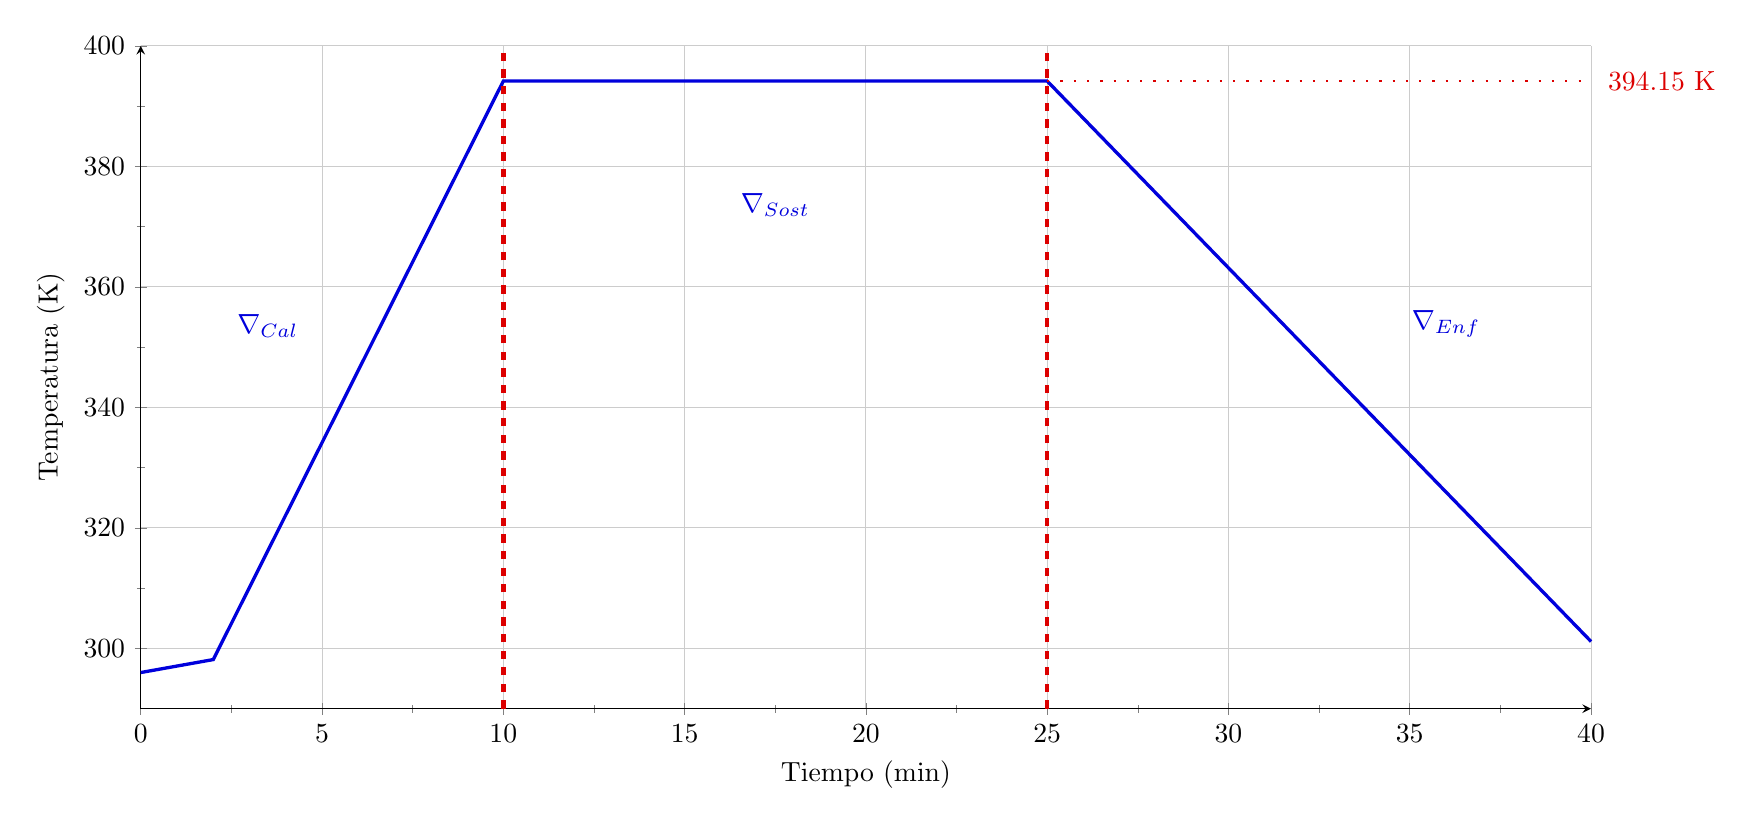
\begin{tikzpicture}
\begin{axis}[
    width=20cm, height=10cm,
    xlabel={Tiempo (min)},
    ylabel={Temperatura (\unit{\kelvin})},
    xmin=0, xmax=40,
    ymin=290, ymax=400,
    xtick={0,5,10,15,20,25,30,35,40},
    ytick={300,320,340,360,380,400},
    yticklabels={300,320,340,360,380,400},
    grid=major,
    major grid style={line width=0.3pt,draw=gray!40},
    minor tick num=1,
    axis lines=left,
    enlargelimits=false,
    clip=false,
    legend pos=south east,
    legend style={draw=gray!50},
]

% Curva de temperatura (en Kelvin)
\addplot[very thick, DarkBlue] coordinates {
    (0,296)
    (2,298.15)
    (10,394.15)
    (25,394.15)
    (40,301.15)
};

% Línea horizontal de referencia 394.15 K (= 121 °C)
\addplot[loosely dotted, thick, DarkRed, domain=25:40] {394.15};
\node[anchor=west, DarkRed] at (axis cs:40.2,394.15) {394.15 \si{\kelvin}};

\addplot[dashed, ultra thick, DarkRed, forget plot] coordinates {(10,290) (10,400)};
\addplot[dashed, ultra thick, DarkRed, forget plot] coordinates {(25,290) (25,400)};

% Anotaciones de fases
\node[anchor=south, DarkBlue, align=center] at (axis cs:3.5,350) {$\nabla_{Cal}$};
\node[anchor=south, DarkBlue, align=center] at (axis cs:17.5,370) {$\nabla_{Sost}$};
\node[anchor=south, DarkBlue, align=center] at (axis cs:36,350) {$\nabla_{Enf}$};

\end{axis}
\end{tikzpicture}
\end{document}